%\documentclass[fontsize=11pt, appendixprefix=true]{scrreprt}
\documentclass[11pt]{report}
\usepackage{tocloft}
%\renewcommand{\cftpartleader}{\cftdotfill{\cftdotsep}} % for parts
%\renewcommand{\cftchapleader}{\cftdotfill{\cftdotsep}} % for content
\renewcommand{\cftsecleader}{\cftdotfill{\cftdotsep}} % for sections, if you really want! (It is default in report and book class (So you may not need it).

% appendixprefix: hogy odaírja, hogy "Függelék A", ne csak "A"
%\usepackage[english, magyar]{babel}                        % nyelvi csomag
\usepackage[T1]{fontenc}                                   % ékezetes betűknél is legyen automatikus elválasztás
\usepackage[utf8]{inputenc}                                % ékezetes betűk kezelése
%\usepackage{lmodern}                                       % alapértelmezett betűtípus ne legyen pixeles
%\usepackage{mathtools}                                     % képletekhez kell
\usepackage[backend=biber, sorting=anyt]{biblatex}           % bibliográfia
\usepackage{parskip}
\addbibresource{projectlab.bib}
\usepackage{url}
\usepackage{enumitem}
\usepackage{amsmath}
\usepackage{amssymb}
\usepackage{graphicx}                                      % képek beszúrása
%\usepackage{subcaption}
\usepackage{subfig}
\graphicspath{ {images/} }
\usepackage[export]{adjustbox}                             % ez az ITK logó pozicionálásához kell
\usepackage[margin=2.5cm, bindingoffset=1.25cm]{geometry}  % margók
\usepackage[onehalfspacing]{setspace}                      % másfeles sorköz
\usepackage[hidelinks, unicode, pdfusetitle]{hyperref}     % kattintható tartalomjegyzék és hivatkozások
\usepackage{bookmark}                                      % PDF könyvjelzők
\usepackage{csquotes}                                      % a bibliográfiában megfelelően legyenek formázva az idézőjelek
\DeclareQuoteAlias{german}{magyar}
\usepackage{blindtext} %mer mért ne?
% Kódrészletekhez ajánlom
\usepackage{listings, scrhack}
%\usepackage{sourcecodepro} % egy jó betűtípus
\lstset{captionpos=b, numberbychapter=false, basicstyle=\ttfamily, showstringspaces=false, columns=fullflexible}
% Kódrészletek magyar stílusú számozása
%\renewcommand\lstlistingname{kódrészlet}
%\makeatletter
%\renewcommand\fnum@lstlisting{\ifx\lst@@caption\@empty\else\thelstlisting.~\fi\lstlistingname}%
%\makeatother
% Nyilatkozathoz két parancs definíciója
\newcommand{\pushtobottom}{\vspace*{\fill}}
\newcommand{\signatureline}[1]{\begin{flushright}
	\vspace*{.5cm}\par\noindent\makebox[2.5in]{\hrulefill}
	\par\noindent\makebox[2.5in][c]{#1}
	\end{flushright}
}

% reference
%\usepackage[plain]{fancyref}
%\usepackage[english, nameinlink]{cleveref}

%formázás

\usepackage{fancyhdr}
\pagestyle{fancy}
\fancyhf{}
%\fancyhead[L]{\leftmark}
\fancyhead[L]{\textsl{\rightmark}}
\fancyhead[R]{\thepage}
\renewcommand{\headrulewidth}{.001cm}

% Ezeket írd át!
\author{Csaba Botos}
\title{
Deep learning framework in TensorFlow\\
for biomedical research
}
\date{2017}

\usepackage{titlesec}

\usepackage{courier}
\lstset{basicstyle=\ttfamily,breaklines=true}
\lstset{framextopmargin=50pt}

% Chapter customization
\renewcommand\thesection{\arabic{section}}
\setcounter{secnumdepth}{2}

\titleformat{\chapter}[block]
  {\normalfont\Huge\bfseries}{\thechapter.}{1em}{\huge}
%\titleformat{\subsection}[block]

% For quotes
\usepackage{epigraph}
\setlength\epigraphwidth{0.7\textwidth}
\setlength\epigraphrule{0pt}

% For multi fig in row
\usepackage{floatrow}

% No page break before chapters
\usepackage{etoolbox}
\makeatletter
\patchcmd{\chapter}{\if@openright\cleardoublepage\else\clearpage\fi}{}{}{}
\makeatother

\begin{document}
%%%%%%%%%%%%%%%%%%%%%%%%%%%%%%%
%% BEVEZETÉS


\includegraphics[valign=m]{ITK_logo} \parbox[c]{\textwidth}{
Pázmány Péter Catholic University\\
Faculty of Information Technology and Bionics}
\vspace*{\fill}

{\let\newpage\relax\maketitle}
\vspace*{\fill}
\begin{center}
A review submitted in partial satisfaction of the requirements of Guided Individual Study.
\bigskip

Advisor: PhD.\ István Z. Reguly \\
\end{center}
\clearpage


\pagenumbering{Roman}
\chapter{Abstract}
Atrial Fibrillation is the most common type of cardiac arythmia.

ötletek még abstracthoz

http://www.sciencedirect.com/science/article/pii/S1746809413000062

https://physionet.org/challenge/2017/

\addcontentsline{toc}{chapter}{Abstract}

\pagenumbering{arabic}
\chapter{Introduction}
\section{Overview}


\epigraph{\textit{No one knows what the right algorithm is, but it gives us hope that if we can discover some crude approximation of whatever this algorithm is and implement it on a computer, that can help us make a lot of progress.}}{\rightline{{\rm --- Andrew Ng}}}

Every time we are interacting with our environment, we get closer to understanding it. %still the closer we are the less we understand. 
However, as a byproduct, further questions arise, for which pure logical (or mathematical) solution is not available, or the problem is larger than what we can solve.
Luckily we can always turn back to nature for inspiration: biological systems have proven their efficiency, therefore their functions are worth to be further analyzed -- even if there could be theoretically a better way to tackle obstacles. 
One of the many branches of artificial intelligence, Neural Networks are based on the nervous systems of living organisms which is capable of self-learning.

Such a simple paradigm is playing a fundamental role in boosting 
industry and research of today, because introducing Machine Learning to many fields of life seems to results in great leap forward. 
Thanks to the recent technological advancements, even with the current computational capacity of a personal computer one can get encouraging results by simply exploring the core principles of the topic. 

In this work I provide a detailed explanation of each step of building a library,
which is capable of reproducing current results of scientific researches.
Also present applications which were made with my own library and case studies in which I have achieved unique results.
Finally I propose the main innovation of my recent work: a simple algorithm for visualizing the \textbf{perceptive field} of each layer in a feed-forward network.

\paragraph{Primary goal.} With my work I intend to bring closer, and demystify cutting-edge concepts of applied neural networkings for larger audiences. 
On related works and case studies I want to show what can be done by simply going back to the drawing board

\clearpage
\section{Related Works and Literature}

\paragraph{Main motivation.} By using external libraries \cite{TF, torch, caffe}, without diving deep into mathematical proofs, and treating neural networks as black-boxes, thousands of useful applications \cite{haykin2004comprehensive} are made. 
On the other hand, building such architectures from the very basics helps to clarify how simple units might be organized~\cite{milo2002network}, taught \cite{werbos1994roots}, and function \cite{hornik1989multilayer} as a large system. 
As complexity arises, the processes in the network becomes unclear and brings the question: what is the purpose of each node? 
Methods to visualize how activation patterns formulate, and what information is held within them has been already investigated \cite{yosinski2015understanding}, and applied to improve performance \cite{zeiler2014visualizing}. 
My studies mainly rely on recent publications, and research in field of computer vision. The design of my own Deep Learning framework library is influenced by off-the-press tutorials \cite{Goodfellow-et-al-2016-Book, deeplearningdotnet, nnsdl, stanfordlectures, gibiansky} and open-source libraries \cite{TF, torch, caffe} available to anyone.

Considering course slides \cite{stanfordlectures, oxfordlectures} and textbooks \cite{Goodfellow-et-al-2016-Book, werbos1994roots, bengio2009learning} of established universities, popular websites \cite{deeplearningdotnet, pedregosa2011scikit}, 
articles \cite{lecun2015deep}, blogs \cite{gibiansky, karpathyblog} and vlogs \cite{vlog1} on Artificial Neural Networks one might find it hard to find a good point to start. 
Some content may offer formal description of the general machine learning problem, others try to clarify through analogies with the biological nerve system.
Tutorials, which I have found interesting, and the most helpful, had several common features which are important to adapt, when designing a neural network library.
Generally these common attributes are the following: 
they intend to be \emph{simple} as possible, 
have many \emph{intuitive} examples and analogies,
their \emph{interpretations} are not restricted to either universal approximators, 
or nervous systems of living organisms, but combines both aspect.

I have written the first implementation based on chapters of \cite{nnsdl}. 
What I have understood is the basic forward- and back-propagation \cite{werbos1994roots} concept of neural networks.
Since I was struggling to understand the coding tricks that the author involved 
I could not extend the source to any problem.
I decided to work out the mathematical formulation, to re-implement feed-forward networks from the beginning.
Reading a practical guide~\cite{karpathyblog} pointed out how can we represent \emph{gradient flow}, \emph{computational graphs} in a simple way.
His style of explaining complex theoretical concepts through very clear examples motivated me to
write my own guide which covers those parts that I was missing from the literature mentioned above.

When the library was working, the next step was writing demo applications, in which I have experimented with hyper-parameters.
These applications were based on \emph{Browser demos} of \cite{convnetjs}.
In this work only two of them is present, which are related to visualization.
Later I was experimenting with different methods of revealing the \emph{perceptive field}.
In \cite{breakingclass} I learned about how modern networks can be fooled with \emph{adversarial samples} which referred to \cite{goodfellow2014explaining} and \cite{nguyen2015deep}. 
Further investigation in the area revealed basic methods on understanding how each neuron works in a network \cite{yosinski2015understanding}.
I was inspired to develop my own algorithm while I was studying the novel architecture of DeconvNets \cite{zeiler2014visualizing}.

\clearpage
\section{Thesis outline and contributions}
In this work I summarize my recent studies on Neural Networks and Computer 
Vision. 
I present my current achievements in the field, the visualization 
techniques I have derived and developed from the latest 
self-educational sources and novel research.
I also provide a guide on how to build a library \textbf{from scratch} 
which I used for producing the present results.


In Chapter \textbf{\nameref{cp:design}} I explain the overall structure of the library and the considerations which led to them, and provide a detailed explanation on how I 
derived the main concepts of neural networks, from the very beginning supported with mathematical background. 
First I zoom in from a larger picture of working AI to exact challenges of 
Machine Learning: I disassemble neural networks in general, to basic 
building blocks, explain them through several examples and provide a 
formal mathematical definition which will be used in the following 
sections.
I put emphasis on linking the formal definitions to natural meanings of 
mathematical formulas (throughout rather informal explanations).
By providing intuitive theoretical considerations, from the perceptron 
model, I build up step-by-step the entire idea of \emph{Forward- \& 
Back-propagation} of Deep Neural Networks.
In the end, exact layers are described involving examples of practical applications.

In \textbf{\nameref{cp:results}}, I describe my research on 
visualization techniques via elementary case studies of \emph{Voice 
Recognition} and \emph{Image Classification}.
In the first half I summarize the main concepts and capabilities of single 
layered neural networks.
I start with the basic problems of voice recognition, namely the 
overlapping frequency domains, the irrelevant signals (noise) by training 
networks on pure sinusoid input samples.
I provide examples for the problem of overfitting and show how regularization techniques enhances the network performance.
After clarification, I explain the challenges of the voice recognition topic involving real recordings,
a case study that can be carried out at home by anyone, with the knowledge 
provided by my work.
In the second half, I show how feed-forward networks can be better understood via visualization with a simple algorithm, namely the \emph{Gradient Ascent}, which I have developed based on my previous studies of novel articles.
I have also explored the hyper-parameter space of fully connected architectures,
while training networks on the popular MNIST dataset.
I present my experiments with different shape of layers and methods for training, and share my interpretations of the results.
In the end an exhaustive investigation of different types of Gradient Ascent can be found involving research of revealing perceptive field of neuron each neuron in a given layer and generating adversarial samples from any kind of input which can be used for harnessing the network.

Finally, in the last chapters I summarize the research I have done so far and discuss the path forward.





%
%\section*{Biological Motivation}
%\section*{Real Life Applications}
%\section*{Black Box representation}
%\section{The Perceptron model}
%\section{Importance of understanding}
%\section{Visualization}


%% BEVEZETÉS
%%%%%%%%%%%%%%%%%%%%%%%%%%%%%%%
%% TARTALOM
\chapter{Related Works}

ez még maradhat a végére


\chapter{My commitments to the project}

I aim to generalize this writing and be less specific about the exact project we are working on, so the following experiences can be transferred to other fields of otherwise non related studies.
Basically our task was a simple classification problem for time samples of various length.
My task was not just to try out famous Machine Learning concepts which \textit{may} work, but to support our research group with the necessary backend of the experiments carried out, and to integrate different results in the final unified model.

\paragraph{Environment.}
For doing so I decided to use TensorFlow environment, in which I had previous experience, i.e.\ in building semantic analyzer for movie dialogs, image classifiers, and text generation for chatbots, image generation using Generative Adversarial Networks etc.
For our project we started by applying different previously proven to be succesful feature extraction methods, and for introducing Deep Learning we wanted to improve our progress by building on top of these features.
So in the first step I had to break down the recent DL architectures I wanted to use to basic modules.
When reimplementing them I paid attention to make spaceholders or entry points for every possible external features my colleagues developed.

Entry points at different level of processing the input can be categorized as the following:
- Variable length features (i.e. output of filters).
- Fixed representation features (i.e. variability indices, frequency domain components).
- Suggestions for classes (i.e. external classifier suggestion)

Also, to improve the model's efficiency I applied queues after different entry points to make mini-batch processing available, by filling these queues independently in mutliple threads, so the network trainer do not have to wait for these external sources to finish their processes to update the network's weights.

\paragraph{Data standardization.}
The biggest obstacles at first sight in using TensorFlow are the Tensors and the (control) Flow itself. In order to deploy a model we have to first assemble its computational graph, which will be compiled at run-time so it can be fed with real NumPy arrays and evaluated in the most efficient way relying on the TensorFlow backend.

Knowing that any time we feed values in, and retreive values from Tensors the whole process has to switch back and forth between C++/CUDA backend and the Python interface, which in case of large arrays is computationally expensive, and possibly collapse the parallel processes to sequential evaluation causing unnecessary run-time overhead, making TensorFlow seemingly inefficient.
In order to achieve best performance we have decrease the number of python API calls of Tensor evaluation, to let the backend order its computations in one run.

Special case of reducing calls is to discard the notorius use of placeholders~\cite{noauthor_performance_nodate, noauthor_tensorflow:_nodate}, and introduce Queues to the model.

TensorFlow comes with a handful of convenience functions and wrappers which can handle data loading and preprocessing in parallel threads, controlled by a native thread coordinator.

These operators can be built in the graph without actually loading the data, and provide Tensor outputs which instead of placeholders will feed the network automatically on evaluation, so we can forget the \textit{feed dict}.
By using queues we can ensure that the main training process is running continously by chopping minibatches off the queues' front while new samples are fed back to the other end, possibly on different devices and multiple threads.
As a result the main process will not starve on input data, neither will be continously interrupted by Python calls to simply just transfer values from the API to the backend.

For the reasons above I prepared a \textit{writer.py} script that takes our raw data files, reads them into memory and write them out in a single file in the suggested file format, \textit{.TFRecord}.
These files can be managed more easily, preserve the sufficient data in a compact way~\cite{noauthor_tfrecords_nodate}, and the most important part, they can be automatically transformed into Tensors.

To make our experiments standardized, we first separated a train and a test set from the original data in 80-20 ratio, and due to unbalanced entries class representation, I wrote and augmentation script to create an evenly sampled pre-training set with a disjunct train and validation set (80-20), in order to prevent the model from learning a single answer for every sample.

\paragraph{Digital Filter.}
Since our original approach was built upon modified Pan Tompkins filtering method~\cite{pan1985real}.
When we refactored our code base to use TensorFlow, we approached a great obstacle: there was no previous work involving filters.
While in SciPy we could reproduce the same results of the original MatLab code~\cite{noauthor_complete_nodate}, the above mentioned problem of feeding external values instead of integrating the process in the computational graph was apparent again.
We had to decide whether we pre-process all sample before writing the 'TFRecords' files keeping the heavy computing outside of our model, or implement the repeatedly used 'filtfilt' operation, and rewrite the method completely using abstract native TensorFlow Tensors and Op nodes.

Considering that we have to deploy the algorithm in real time inference application, we choose the latter.
As a first step, my colleagues reimplemented the method using NumPy, that I used as a template to follow while writing a new basic TF operator called 'lfilt'.
I paid attention to keep the TF policy which is that operators borrowed from SciPy and NumPy should be transparent by function call signature, and the output should behave the same way as in the original implementation.


- FeedBack filter components:   $A = a_0, a_1, a_2 \dots a_M$, where $a_0 = 0$ by definition
- FeedForward filter components:   $B = b_0, b_1, b_2 \dots b_N$

\begin{lstlisting}[language=Python]
# Lfilt operation definition at time step `t`
y(t) = x(t)*b(0) + x(t-1)*b(1) + x(t-2)*b(2) ... x(t-M)*b(N)
                       - y(t-1)*a(1) - y(t-2)*a(2) ... y(t-N)*a(M)
\end{lstlisting}

$$
y_t = \sum_{i=0}^{N} x_{t-i} \cdot b_{i} - \sum_{i=1}^{M} y_{t-i} \cdot a_{i}
$$


\begin{lstlisting}[language=Python]
y(t) = x[t-N : t] * b[::-1] - y[t-M : t-1] * a[::-1]
\end{lstlisting}


for faster computation let $s$ be $s := x \ast b$, where $\ast$ is the convolution operator. This can be evaluated previusly at once since all values of $x$ is known at computation time

\begin{lstlisting}[language=Python]
y(t) = s[t] - y[y-t : t-1] * a[::-1]
\end{lstlisting}

As in the SciPy source code we can see~\cite{noauthor_scipy/scipy_nodate}, on lfilt calls both $A$ and $B$ are expected to include the $0^{th}$ parameter as well, which in the feedback operator's case will mean that in the exact computation we have to normalize both $A$ and $B$ by $A_0$ and leave out the $0^{th}$ component from $A$, since it is the corresponding constant of the current $y_t$ value.

\paragraph{Visualization.}
We always have to keep track, of what we have tried before, and after dozens of runs of experiments it is only up to us what we logged, and how well can we remember.
To make a decision on future steps in the project it is always useful if we can avoid crawling through a messy git history to find the actual train scripts we wrote, then start to extract the hyperparameters from the code - it uses up a tremendous time, and chances of missing something is very high.

To make debugging, optimization, and workgroup meetings productive, I used TensorBoard, that is able to read native TensorFlow log or \textit{summary} files and automatically turns them into spectacular graphs (see Figure \ref{fig:tf-graph} and \ref{fig:hist}), and quantitative metrics (see Figure \ref{fig:tf-score}).
The more explicit name and variable scopes we include in our code the more detailed the resulting graph and scorings will be.

\begin{figure}[h]
  \centering
  \includegraphics[width=\textwidth]{tf-graph}
  \caption{Left: Inner structure of a FCN. Right: The \textit{Confusion Matrix} operator is build using elementary TensorFlow operations.}
  \label{fig:tf-graph}
\end{figure}

\begin{figure}[h]
  \centering
  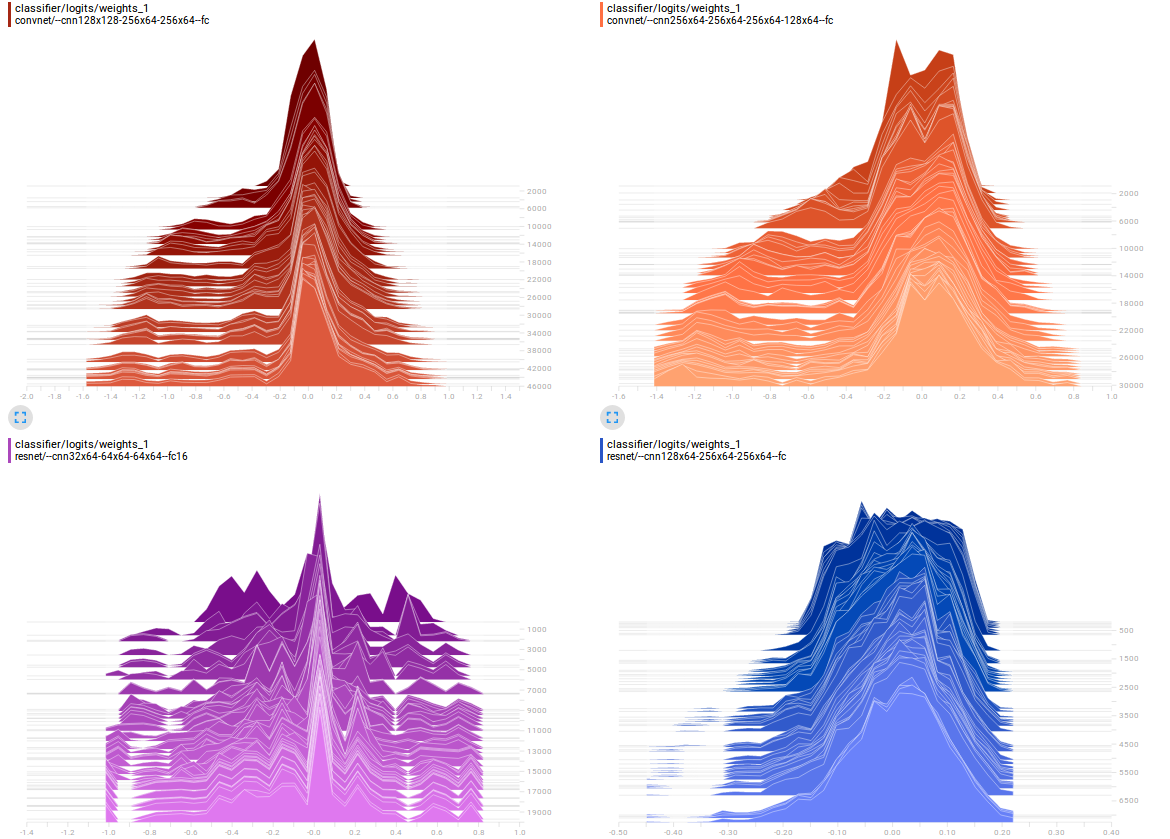
\includegraphics[width=\textwidth]{hist}
  \caption{Using histograms we can keep track of our model's progress during the training session. We may look for local pikes in the distribution of the layers' weights, or biasing toward a specific mean through time.}
  \label{fig:hist}
\end{figure}

\begin{figure}[h]
  \centering
  \begin{floatrow}
    \ffigbox[\FBwidth]{\caption{Performance test of Deep Residual networks}}{%
      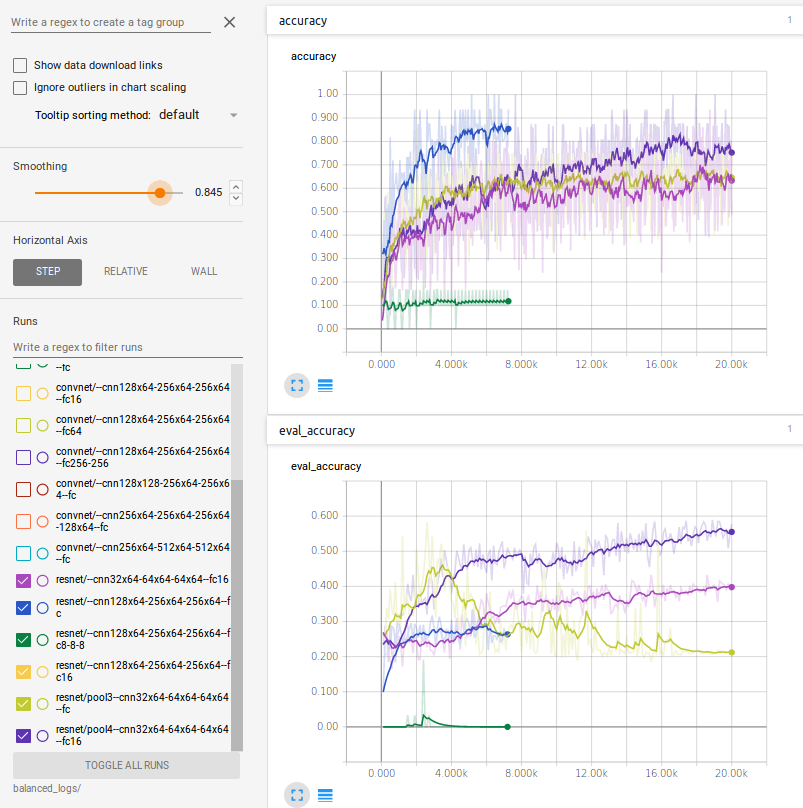
\includegraphics[width=.48\textwidth]{resnet-overall}
    }
    \ffigbox[\FBwidth]{\caption{Performance of Fully Convolutional networks}}{
      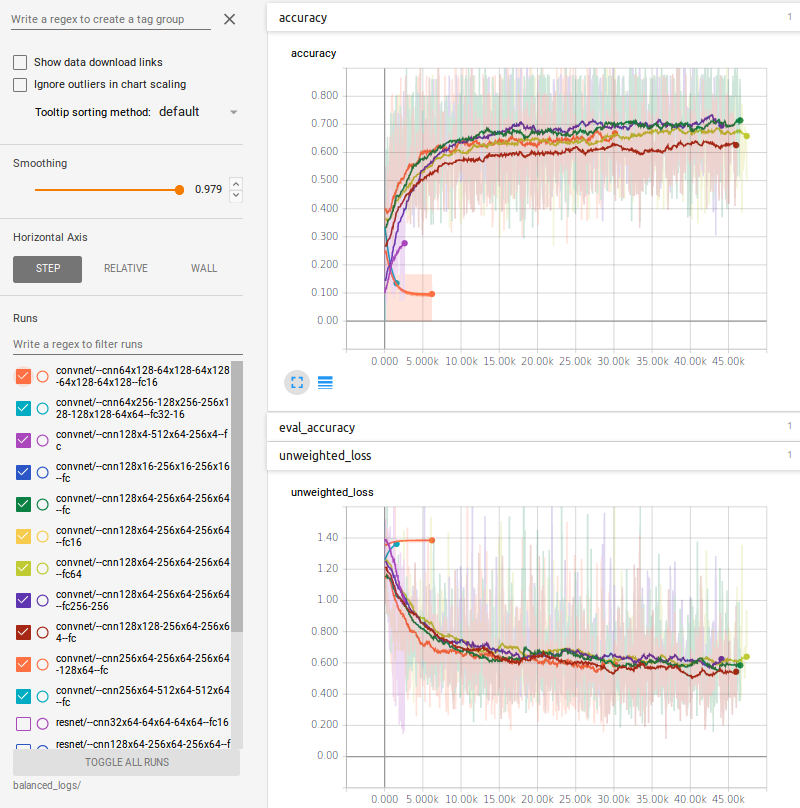
\includegraphics[width=.48\textwidth]{convnet-overall}
    }
  \end{floatrow}
  \label{fig:tf-score}
\end{figure}

By utilizing TensorBoard we boosted our progress, because we could easily determine if a training should be stopped because the network collapsed, track down which layer was causing this failure by investigating the forward and backward pass of activations and gradients, the distribution of the models variables grouped by layers - all in all whether an experiment branch should be further investigated or not.

\paragraph{Fast prototyping.}
To make our experiments easily reproducible I refactored our network modules to be able to build themselves by just simply using a few high level hyperparameters, just like as number of internal layers, capacity, reduction factor (av/max pooling), etc. and made a template \texttt{.json} file which held these prototype variables, allowing us to use the same training script to build and train a wide variety of different architectures while saving and logging them in high detail to separate directories.

When servers with multiple GPUs are available, we can also boost our fine-tuning phase, with running trainings on parallel threads.
By default a single TensorFlow session allocates the whole GPU source, even if the graph is not able to use but a single unit.
So for parallel tests, I wrote a shell program with which we can launch the training with different parameters, automatically reserving the required devices to each training and restricting it from interfering in other processes.


%% TARTALOM
%%%%%%%%%%%%%%%%%%%%%%%%%%%%%%%
%% BEFEJEZÉS
\chapter{Benchmark of \texttt{filtfilt}}

In order to verify that my implementation of the \texttt{filtfilt} operator in TensorFlow is better for large scale applications than the publicly available state-of-the art method found in \texttt{SciPy.signal module}~\cite{scipy}, we attempted to measure the time required for evaluation.
For benchmarking purposes we used random sequences sampled from standard normal distribution.

I have prepared multiple test runs, where we compare the two methods by evaluation time concerning the sample length, the number of filters applied and the number of samples.

\section{Single sample - Single filter with different sample lengths}
In the first comparison the TensorFlow implementation performs poorly, we had to apply different $y$ label ticks.
The reason for this result, is that the implementation uses GPU acceleration via TensorFlow CUDA kernels, and the mobilization of the data (copying into the graphic memory, and copying the result out from it) takes more time than actually executing the operation.
Moreover, currently the TensorFlow backend does not support mutable \texttt{tf.Variables} inside native iterative loops \texttt{tf.while\_loop}, meaning that we cannot modify specific values by indexing an immutable \texttt{tf.Tensor}.
 In other words, \texttt{tf.Tensor} is the only interface for the inner body of the while loop that can communicate with external graph nodes.
Technically this yields, that the fixed size array of values cannot be allocated before the execution of an iteration, because the resulting space can only be handled by an interface that does not support element modification.
As a transient solution we had to include array concatenation, so in every step $t$ the array of previous outputs $[y_{1}, y_{t-1}]$ has to be concatenated to the current $y_t$ output value, resulting in memory expensive operations.

\begin{figure}[h]
  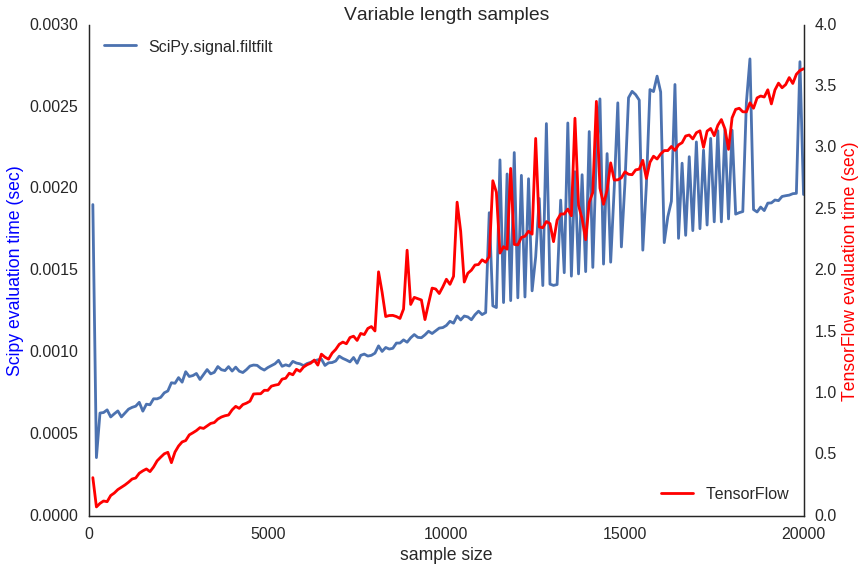
\includegraphics[width=.9\textwidth]{single}
  \caption{Time of evaluating a single sample with a single filter, at different sequence lengths. Later the measurement depicted with the blue line will be used as a baseline representing SciPy's performance on the given task. Notice that for we introduced a new axis for the TensorFlow implementation's time scale, because on single samples the performance of the two methods were not comparable.}
\end{figure}

\section{Batch of samples - Single filter run, with same length samples}

When multiple samples are available at run time, we can speed up the process, by running the same filter process in parallel.
Here we normalized the evaluation time per sample per filter of the SciPy method using the statistics of the previous experiment, since the method allows only processing in sequence, and after reproduced the standard SciPy baseline, to use as a reference point in further benchmarks, e.g. Figure~\ref{fig:batch}.
As we can see in Figure~\ref{fig:batch-tf-only}, the TensorFlow implementation runs in constant time at low batch size, and later starts to increase linearly

\begin{figure}
  \centering
  \begin{floatrow}
    \ffigbox[\FBwidth]{\caption{Comparison to the standardized SciPy baseline with regards to the baseline. The baseline is computed from the normalized average of the different sample length runs from the variable length single sample experiment. We show that with sample length 100, the current implementation only functions better when evaluation above 1500 sample at once.}\label{fig:batch}}{%
      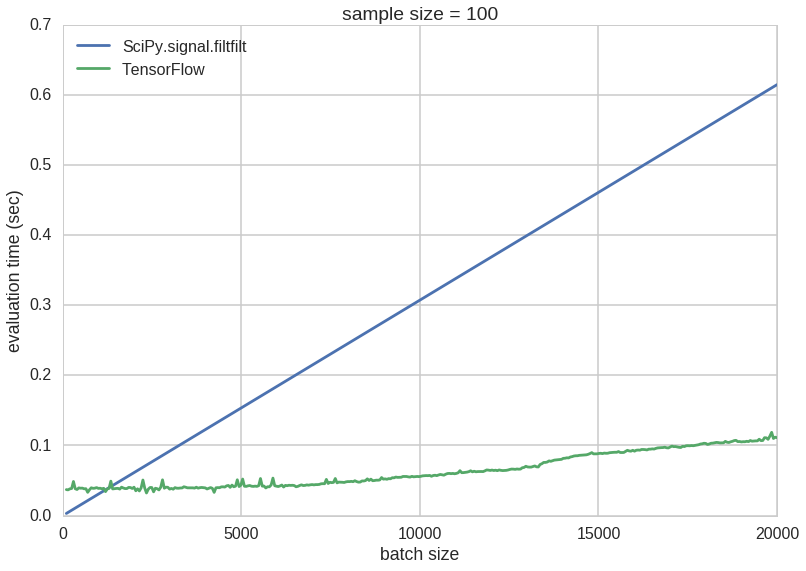
\includegraphics[width=.48\textwidth]{batch}
    }
    \ffigbox[\FBwidth]{\caption{Here only the TensorFlow implementation's evaluation time is depicted without the baseline. It reveals that under 4000 samples the process is nearly constant in time complexity. Above 2000 samples it starts to behave linearly, but it is important to mention that the slope of the fitting linear curve is significantly less steeper than the SciPy baseline.}\label{fig:batch-tf-only}}{%
      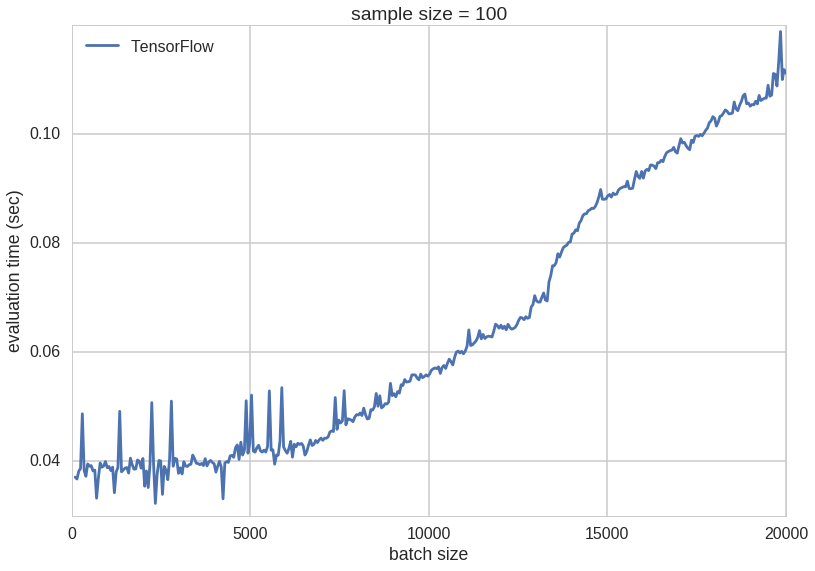
\includegraphics[width=.48\textwidth]{batch-tf-only}
    }
  \end{floatrow}
\end{figure}

% \begin{figure}
%   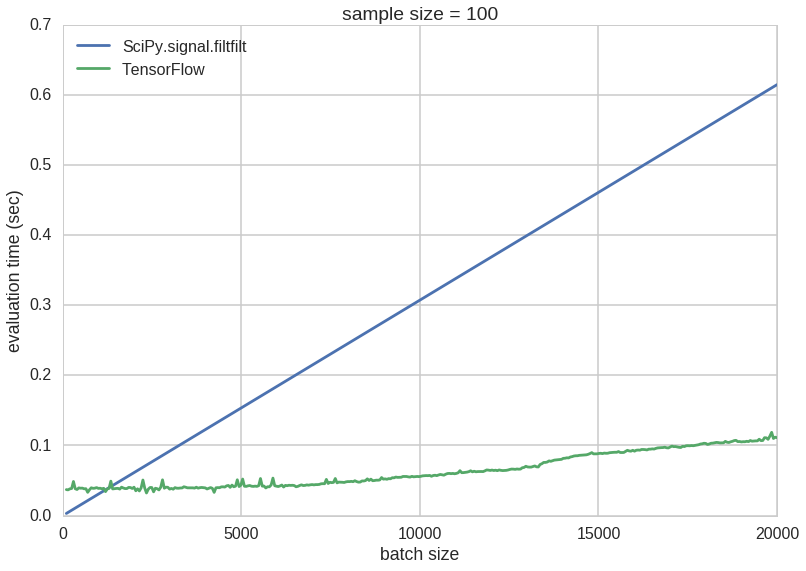
\includegraphics[width=.9\textwidth]{batch}
%   \caption{Comparison to the standardized SciPy baseline with regards to the baseline. The baseline is computed from the normalized average of the different sample length runs from Section~\ref{sec:single}}
%   \label{fig:batch}
% \end{figure}

% \begin{figure}
%   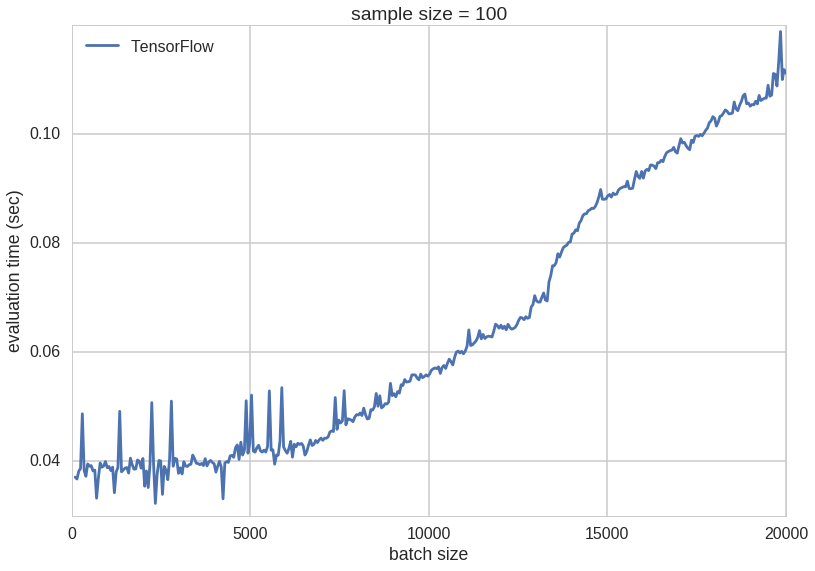
\includegraphics[width=.9\textwidth]{batch-tf-only}
%   \caption{Here only the TensorFlow implementation's evaluation time is depicted without the baseline. It reveals that under 2000 samples the process is nearly constant in time complexity. Above 2000 samples it starts to behave linearly, but it is important to mention that the slope of the fitting linear curve is significantly less steeper than the SciPy baseline.}
%   \label{fig:batch-tf-only}
% \end{figure}

\section{Time per sample}
Finally, we normalized the computation time with regards to the batch size, as a result we have a curve that tells that with fixed sample length at given batch size how much time does it take to evaluate a single entry. For a detailed benchmark see Figure \ref{fig:norm}.

\begin{figure}
  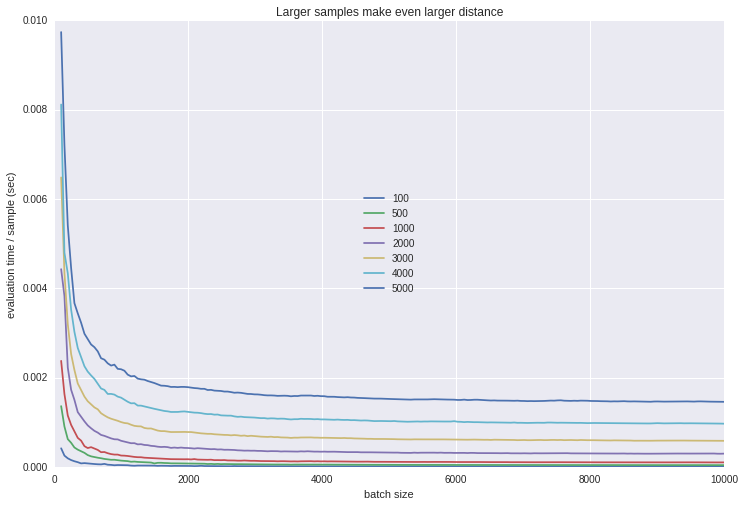
\includegraphics[width=.9\textwidth]{norm}
  \caption{This curve tells that with fixed sample length (different curves on the figure) at given batch size how much time does it take to evaluate a single entry.}
  \label{fig:norm}
\end{figure}


\chapter{Future}

\paragraph{Short-term plans.} 
Currently I have a working version of the convolutional layer, 
however the implementation still relies on \texttt{convolve2d} function of ScyPy, which slows down the training process.
In the following months I will work on my own implementation of the convolution function, 
and improve the network usability.
Recently I have been able to train my network on CIFAR~\cite{cifar}, and ImageNET~\cite{deng2009imagenet} dataset, and the results are encouraging, however not enough yet to publish.
I am also working on \emph{Restrictive Boltzmann Machines} to be able to build and make experiments of \emph{Deep Belief} networks.

I am very interested in fields of \emph{Reinforcement Learning}, 
and I plan to utilize a network that plays the popular game, \texttt{agar-io}.
Also I am currently studying \emph{Recurrent Neural Networks} especially implementations of \emph{Long Short-Term Memory} architectures, 
which are not just better for audio recognition tasks, but can be used as Generative networks, producing artificial samples.
I want to create an application capable of accompanying musicians in jam-sessions, based on \emph{LSTM} networks.
I will continue my studies in field of \emph{Generative Adversarial Networks} which is currently a very hot topic of Computer Vision.

\paragraph{Long-term plans}
My studies have two basic motivation:
When observing living organisms I think about how could we model them, 
and reverse-engineer their function. 
On the other hand, I want to get closer to understand our 
environment and how can we build knowledge based on our experiences.
I believe, that one day my studies in Neuroscience and Artifical Intelligence will converge to a common point, and I will be able to model cognitive functions of the human mind.

\clearpage

\listoffigures
\addcontentsline{toc}{chapter}{List of Figures}
\clearpage

\printbibliography
\addcontentsline{toc}{chapter}{Bibliography}
\clearpage
%% BEFEJEZÉS
%%%%%%%%%%%%%%%%%%%%%%%%%%%%%%%
\end{document}
